\label{chapt:standards}

In this section, well known standards will be investigated.

\begin{itemize}
    \item American Society of Mechanical Engineers (ASME):
	    \begin{itemize}[label=$\bullet$]
	    	\item Boiler and Pressure Vessel Code, Section VIII, Division 1, 2015 \citep{ASMEbvpcVII1}
	    	\item Boiler and Pressure Vessel Code, Section VIII, Division 2, 2015 \citep{ASMEbvpcVII2}
%	    	\item Boiler and Pressure Vessels for Human Occupancy
	    \end{itemize}
	\item Det Norske Veritas(DNV) \citep{DNVOSD101}
		    \begin{itemize}[label=$\bullet$]
	    	\item DNV-OS-D101, Marine and Machinery Systems and Equipment\citep{ASMEbvpcVII1}
	    \end{itemize}
    \item European Standard EN
        \begin{itemize}[label=$\bullet$]
	       	\item EN 13445-3:2014 \citep{EN134453}
	    \end{itemize}
\end{itemize}

%%----------------------------------------------------------------------------------------------------------------------
\section{ASME's BPVC}

\subsection{Section VIII: Division 1}
As per UG-28 of \citep{ASMEbvpcVII1}, the following procedure was used to calculate the required thickness.
The following list of steps were carried out as per \citep{ASMEbvpcVII1}.

\begin{enumerate}
	\item Assume initial thickness value of $t$
	\item Calculate $D_o/t$ ratio and assure $D_o/t \geq 10$.
	\item Calculate $L/D_o$ ratio, if $L/D_o \geq 50 \Rightarrow 50$ or  $L/D_o \leq 0.05 \Rightarrow 0.05$
	\item With above ratios, go to Figure G of \citep{ASMEbvpcIID} and get value for $A$
	\item With $A$ from above go to chart CS-2 $\because S_y \geq 30 \ ksi$ to get $B$
	\item Using $B$ use Equation \ref{eq:2_VII_1_stp6} to calculate allowable pressure $p_a$:
		\begin{equation}
			\label{eq:2_VII1_stp6}
			p_a = \frac{4B}{3 \left(\frac{D_o}{t} \right)}
		\end{equation}
	\item Check if $p_a \geq p_{req}$ as calculated from \ref{eq:2_preq}, if not, incease $t$ and go to Step 1\\
	
\end{enumerate}

With the Python Script in REFAPPENDIX the convergence plot from Figure~\ref{fig:2_vii1_cnvg} below was created.
\begin{figure}[!htbp]
    \centering
    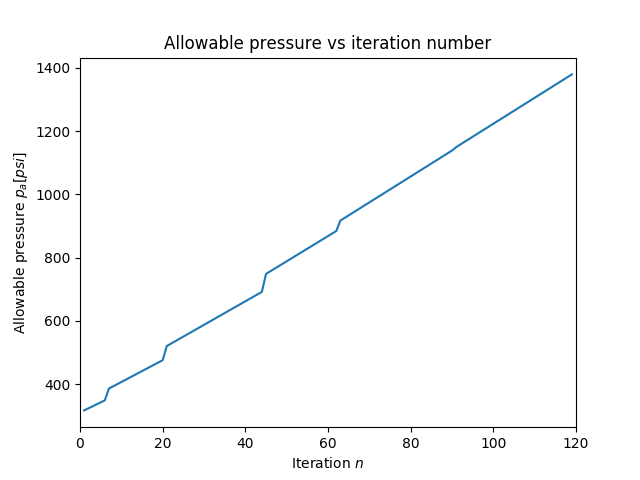
\includegraphics[]{2_vii1_cnvg}
    \caption{Convergence plot of $p_a$.}
    \label{fig:2_vii1_cnvg}
\end{figure}

The script converged at thickness of $t = 1.68\ in$ and an allowable pressure of $p_a~= 1379.4\ psi$ after 119 iterations. 


\subsection{Section VIII: Division 2}
As per subsection 4.4.5 of \citep{ASMEbvpcVII2}, the following procedure was used to calculate the required thickness. Note that only the main formulas will be presented. For intermediate steps, see REFAPPENDIX X for Python script utilized during iteration.The following list of steps were carried out as per \citep{ASMEbvpcVII2}.

\begin{enumerate}
	\item Assume initial thickness value of $t$
	\item Calculate elastic buckling stress $F_{he}$ with \ref{eq:2_VII2_4419}
		\begin{equation}
			\label{eq:2_VII2_4419}
			F_{he} = \frac{1.6\ C_h E_y t}{D_o}
		\end{equation}
	\item Based on $S_y$ and $F_{he}$, calculate the predicted buckling stress $F_{ic}$
	\item With subsection 4.4.2 of \citep{ASMEbvpcVII2}, compute the design factor $FS$
	\item Calculate allowable pressure $p_a$ with \ref{eq:2_VII2_4428}
		\begin{equation}
			\label{eq:2_VII2_4428}
			p_a = 2 F_{ha} \left(\frac{t}{D_o}\right)
		\end{equation}
	\item Check if $p_a \geq p_{req}$ as calculated from \ref{eq:2_preq}, if not, increase $t$ and go to Step 1 \\
	
\end{enumerate}

With the Python Script in REFAPPENDIX the convergence plot from Figure~\ref{fig:2_vii2_cnvg} on page~\pageref{fig:2_vii2_cnvg} was created.
\begin{figure}[!htbp]
    \centering
    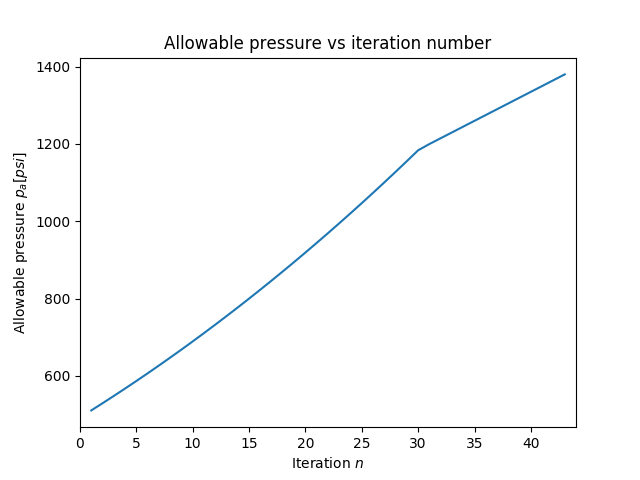
\includegraphics[]{2_vii2_cnvg}
    \caption{Convergence plot of $p_a$.}
    \label{fig:2_vii2_cnvg}
\end{figure}

The script converged at thickness of $t = 0.92\ in$ and an allowable pressure of $p_a = 1379.7\ psi$ after 43 iterations. 


%%----------------------------------------------------------------------------------------------------------------------
\section{DNV}

\subsection{DNV-OS-D101}

As per \citep{DNVOSD101}, in subsection F215, Equation~\ref{eq:2_DNV_hoop} is presented as follows.

\begin{equation}
	\label{eq:2_DNV_hoop}
	\sigma_h = C\cdot\frac{T}{d_{thr}t}
\end{equation}

In this equation, $C$ is a factor based on the number of wraps on the drum,. for two layers $C=1.75$. It is also to be noted that the hoop stress is limited to $\sigma_h \leq 0.85\cdot S_y$. \\

For this application, rearranging for $t$, setting $\sigma_h = S_{allow}$ and solving accordingly will yield a valid value of $t = 1.44 \ in$. 


%%----------------------------------------------------------------------------------------------------------------------
\section{European Standard}
\subsection{EN-13445-3}
As per subsection 8.5.2.2 of \citep{EN134453}, the following procedure was used to calculate the required thickness $e_a$.

\begin{enumerate}
	\item Assume initial thickness value of $e_a$ and calculate $p_y$ with \ref{eq:2_EN_py}
		\begin{equation}
			\label{eq:2_EN_py}
			p_y = \frac{\sigma_e e_a}{R}
		\end{equation}
	\item Compute the lower failure pressure $p_m$ \ref{eq:2_EN_pm}, see 8.5.2.6 of \citep{EN134453} for $\epsilon$
		\begin{equation}
			\label{eq:2_EN_pm}
			p_m = \frac{E e_a  \epsilon}{R}
		\end{equation}
	\item Check if $p \geq p_{req}$ as calculated from \ref{eq:2_preq}, if not, increase $e_a$ and go to Step 1 \\
\end{enumerate}

	
With the Python Script in REFAPPENDIX the convergence plot from Figure~\ref{fig:2_en13445_cnvg}.
\begin{figure}[!htbp]
    \centering
    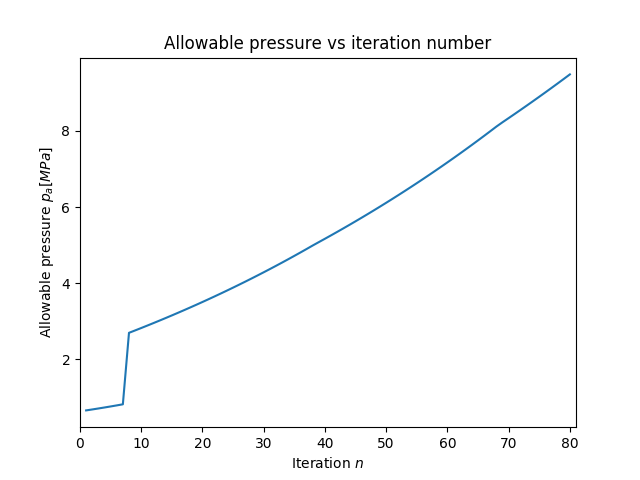
\includegraphics[]{2_en13445_cnvg}
    \caption{Convergence plot of $p_a$.}
    \label{fig:2_en13445_cnvg}
\end{figure}


The script converged at thickness of $e_a = 32.8\ mm$ and an allowable pressure of $p = 9.486\ MPa$ after 80 iterations. 
%%----------------------------------------------------------------------------------------------------------------------
\section{Comparison}

Based on the above sections, the results are summarized in Table~\ref{table:2_comp}.
\begin{table}[htbp]
  \centering
  \caption{Comparison $t$ according to method used.}
    \begin{tabular}{lccc}
          & \multicolumn{2}{c}{\textbf{Results}} &  \\
    \textbf{Method} & \textbf{mm} & \textbf{in} & \textbf{SF} \\
    ASME BPVC VII-1 & $43.2$  & $1.700$ & $1.5$ \\
    ASME BPVC VII-2 & $23.4$  & $0.920$ & $1.5$ \\
    DNV-OS-D101 & $36.6$  & $1.440$ & $1.5$ \\
    EN 13445-3 & $32.8$  & $1.290$ & $1.5$ \\
    \end{tabular}%
  \label{table:2_comp}%
\end{table}%

